\documentclass[a4paper,slidestop,xcolor=pst,dvips,blue]{beamer}

\usepackage{beamerthemesplit}
\usepackage[utf8]{inputenc}
\usepackage[spanish]{babel}
\usepackage{graphicx}
\usepackage{pstricks} % PSTricks package
\usepackage{setspace}
\usepackage{multirow}
\usepackage{listings}
\usepackage{pgfpages}
\usepackage{hyperref}
\usepackage{etoolbox}
\usepackage{epstopdf}

\makeatletter
\patchcmd{\beamer@sectionintoc}{\vskip1.5em}{\vskip0.5em}{}{}
\makeatother

\setbeamercovered{dynamic}
\setcounter{tocdepth}{2}
\setbeamercolor{frametitle}{fg=black,bg=white}
\setbeamercolor{section in toc shaded}{fg=black}
\setbeamercolor{section in toc}{fg=red}
\setbeamercolor{subsection in toc shaded}{fg=black}
\setbeamercolor{subsection in toc}{fg=red}
\setbeamerfont{section in toc}{size=\small}
\setbeamerfont{subsection in toc}{size=\small}
\setbeamertemplate{section in toc shaded}[default][99]
\setbeamertemplate{subsection in toc shaded}[default][99]

\AtBeginSection[]
{\begin{frame}[c]
  \frametitle{Índice}
	\tableofcontents[currentsection,
        sectionstyle=show/shaded,
        subsectionstyle=hide]
\end{frame}}

\AtBeginSubsection[]
{\begin{frame}[c]
	\frametitle{Índice}
	\tableofcontents[
  		currentsection,
  		sectionstyle=shaded/shaded,
  		currentsubsection,
  		subsectionstyle=show/shaded/hide
		]
\end{frame}}

\setbeamercolor{frametitle}{fg=black,bg=white}

\setbeamertemplate{frametitle}{
	\begin{centering}
		\insertframetitle
		\par
	\end{centering}
}

\usetheme[secheader]{Boadilla}

\usepackage{listings}

\definecolor{pblue}{rgb}{0.13,0.13,1}
\definecolor{pgreen}{rgb}{0,0.5,0}
\definecolor{pred}{rgb}{0.9,0,0}
\definecolor{pgrey}{rgb}{0.46,0.45,0.48}

\lstset{language=Java,
  showspaces=false,
  showtabs=false,
  breaklines=true,
  showstringspaces=false,
  breakatwhitespace=true,
  commentstyle=\color{pgreen},
  keywordstyle=\color{pblue},
  stringstyle=\color{pred},
  basicstyle=\ttfamily,
  keywordsprefix={@}
}


\title[Patrones de SIE]{Patrones para el Desarrollo de Arquitecturas Empresariales}

\author[P. Sánchez]{\alert{Pablo Sánchez}}

\institute[IIE]{
		   Dpto. Ingeniería Informática y Electrónica \\
		   Universidad de Cantabria \\
		   Santander (Cantabria, España) \\
		   \texttt{p.sanchez@unican.es}
}

\date{}

\begin{document}

\begin{frame}[c]
	\titlepage
	\begin{columns}
		\column{0.50\linewidth}
			\centering
    		
\includegraphics[width=.28\textwidth,keepaspectratio=true]{images/istr.eps}
		\column{0.50\linewidth}
			\centering
			
\includegraphics[width=.25\textwidth,keepaspectratio=true]{images/uc.eps}
	\end{columns}
\end{frame}

\begin{frame}[c]
    \frametitle{\alert{Advertencia}}
    \begin{center}
        Todo el material contenido en este documento no constituye en modo alguno una obra de referencia o apuntes oficiales mediante el cual se puedan preparar las pruebas evaluables necesarias para superar la asignatura. \ \\
        \ \\
        Este documento contiene exclusivamente una serie de diapositivas cuyo objetivo es servir de complemento visual a las actividades realizadas en el aula para la transmisi{\'o}n del contenido sobre el cual versar{\'a}n las mencionadas pruebas evaluables.  \ \\
        \ \\
        Dicho de forma m{\'a}s clara, \alert{estas transparencias no son apuntes y su objetivo no es servir para que el alumno pueda preparar la asignatura.}
    \end{center}
\end{frame}

\section{Introducción}

\begin{frame}[c]
    \frametitle{Objetivos del Tema}
    \begin{enumerate}[<+->]
         \item Comprender qué es un \emph{Sistema de Información Empresarial (SIE)}.
         \item Comprender cómo y por qué se divide un SIE en capas.
         \item Comprender los patrones arquitectónicos utilizados por un SIE.
         \item Comprender la función de cada capa de un SIE.
         \item Conocer las tecnologías sw que se utilizan para implementar SIE.
         \item Comprender los patrones relacionados con la \emph{capa de negocio}.
         \item Saber utilizar la metodología \emph{Domain-Driven Design (DDD)}.
         \item Comprender el problema de la impedancia objeto-relacional.
         \item Saber utilizar los patrones relacionados con la \emph{capa de persistencia}.
         \item Saber utilizar los patrones relacionados con la \emph{capa de servicio}.
         \item Conocer los patrones relacionados con la \emph{capa de presentación}.
    \end{enumerate}
\end{frame}

\begin{frame}[c]
    \frametitle{Bibliografía}
    \begin{thebibliography}{1}

        \bibitem[Fowler, 2002]{Fowler2002x}
        Fowler, M. (2002).
        \newblock {\em {Patterns of Enterprise Application Architecture}}.
        \newblock Addison-Wesley Professional.

        \bibitem[Evans, 2003]{Evans2003x}
        Evans, E. (2003).
        \newblock {\em {Domain-Driven Design}}.
        \newblock Addison-Wesley Professional.

        \bibitem[Esposito and Saltarello, 2014]{Esposito2014x}
        Esposito, D. and Saltarello, A. (2014).
        \newblock {\em {Microsoft .NET - Architecting Applications for the
          Enterprise}}.
        \newblock Microsoft Press. 2ª Ed.

    \end{thebibliography}
\end{frame}

\section{Arquitectura de los Sistemas de Información Empresarial}

\subsection{Sistemas de Información Empresarial}

\begin{frame}[c]
    \frametitle{Sistema de Información Empresarial}
    %% TODO: Buscar una definición mejor o más estandarizada.
    \begin{block}{Sistema de Información  Empresarial (SIE)}
        Un \emph{Sistema de Información Empresarial} es un sistema sw que da soporte a diferentes procesos de negocio de una determinada organización.
    \end{block}
\end{frame}

\begin{frame}[c]
    \frametitle{Características de los SIEs}
    \begin{enumerate}[<+->]
        \item Necesita almacenar datos, y normalmente, en gran volumen.
        \item Los datos que almacenan representan un activo importante y duradero en el tiempo.
        \item Los gestión de los datos debe obedecer a ciertas \emph{reglas de negocio}.
        \item Las operaciones ejecutadas necesitan ser \emph{transaccionales}.
        \item Los datos pueden ser accedidos y manipulados de manera concurrente.
        \item Utilizan un gran número de interfaces de usuario que pueden requerir de sistemas avanzados de visualización de datos.
        \item Interoperan con otros Sistemas de Información Empresarial.
    \end{enumerate}
\end{frame}

\subsection{Patrones Arquitectónicos de un SIE}

\subsubsection{Arquitectura Cliente-Servidor}

\begin{frame}[c]
    \frametitle{Arquitecturas Cliente/Servidor - Principio Básico}
    \begin{block}{Arquitecturas Cliente/Servidor}
        \begin{itemize}[<+->]
            \item Existe un nodo especializado denominado \emph{servidor}.
            \item El servidor centraliza ciertos cómputos del sistema.
            \item Los clientes realizan peticiones al servidor, el cual las procesa y devuelve las respuesta a los clientes.
        \end{itemize}
    \end{block}
\end{frame}

\begin{frame}[c]
	\frametitle{Arquitecturas Cliente/Servidor}
	\begin{center}
        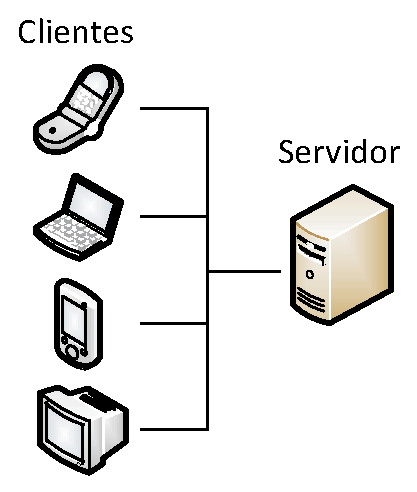
\includegraphics[width=.5\linewidth,keepaspectratio=true]{images/patterns/clienteServidor.eps}
	\end{center}
\end{frame}

\begin{frame}[c]
    \frametitle{Arquitecturas Client/-Servidor - Beneficios}
    \begin{enumerate}[<+->]
        \item Ubicuidad del sistema.
        \item Facilidad de mantenimiento y actualización.
        \item Eliminación de redundancias y posibles inconsistencias.
        \item Permite aligerar los necesidades hardware de los clientes.
        \item Permite trabajar con clientes heterogéneos.
    \end{enumerate}
\end{frame}

\begin{frame}[c]
    \frametitle{Arquitecturas Cliente-Servidor - Problemas}
    \begin{enumerate}[<+->]
        \item Efecto estrella de la muerte.
        \item Necesidad de tener conexión con el servidor.
        \item Problemas de escalabilidad y rendimiento del servidor.
        \item Saturación de las redes de comunicación.
    \end{enumerate}
\end{frame}

\subsubsection{Patrón Código Móvil}

\begin{frame}[c]
    \frametitle{Código Móvil - Principio Básico}
    \begin{block}{Arquitecturas con Código Móvil}
        Un computador (genera y) almacena código y/o datos que se envían a otros computadores para su ejecución.
    \end{block}
\end{frame}

\begin{frame}[c]
    \frametitle{Arquitecturas con Código Móvil - Beneficios}
    \begin{enumerate}[<+->]
        \item Permite distribuir y equilibrar la carga de trabajo.
        \item Utilización y composición de recursos bajo demanda.
        \item Permite aumentar la disponibilidad y tolerancia a fallos del sistema.
        \item Facilitar el mantenimiento y la evolución del sistema.
        \item Ubicuidad de ciertas funciones del sistema.
    \end{enumerate}
\end{frame}

\begin{frame}[c]
    \frametitle{Arquitecturas con Código Móvil - Problemas}
    \begin{enumerate}[<+->]
        \item Agujeros de seguridad.
        \item Saturación de las redes de comunicación.
    \end{enumerate}
\end{frame}

\subsubsection{Arquitectura en Capas}

\begin{frame}[c]
	\frametitle{Arquitecturas en Capas}
	\begin{center}
        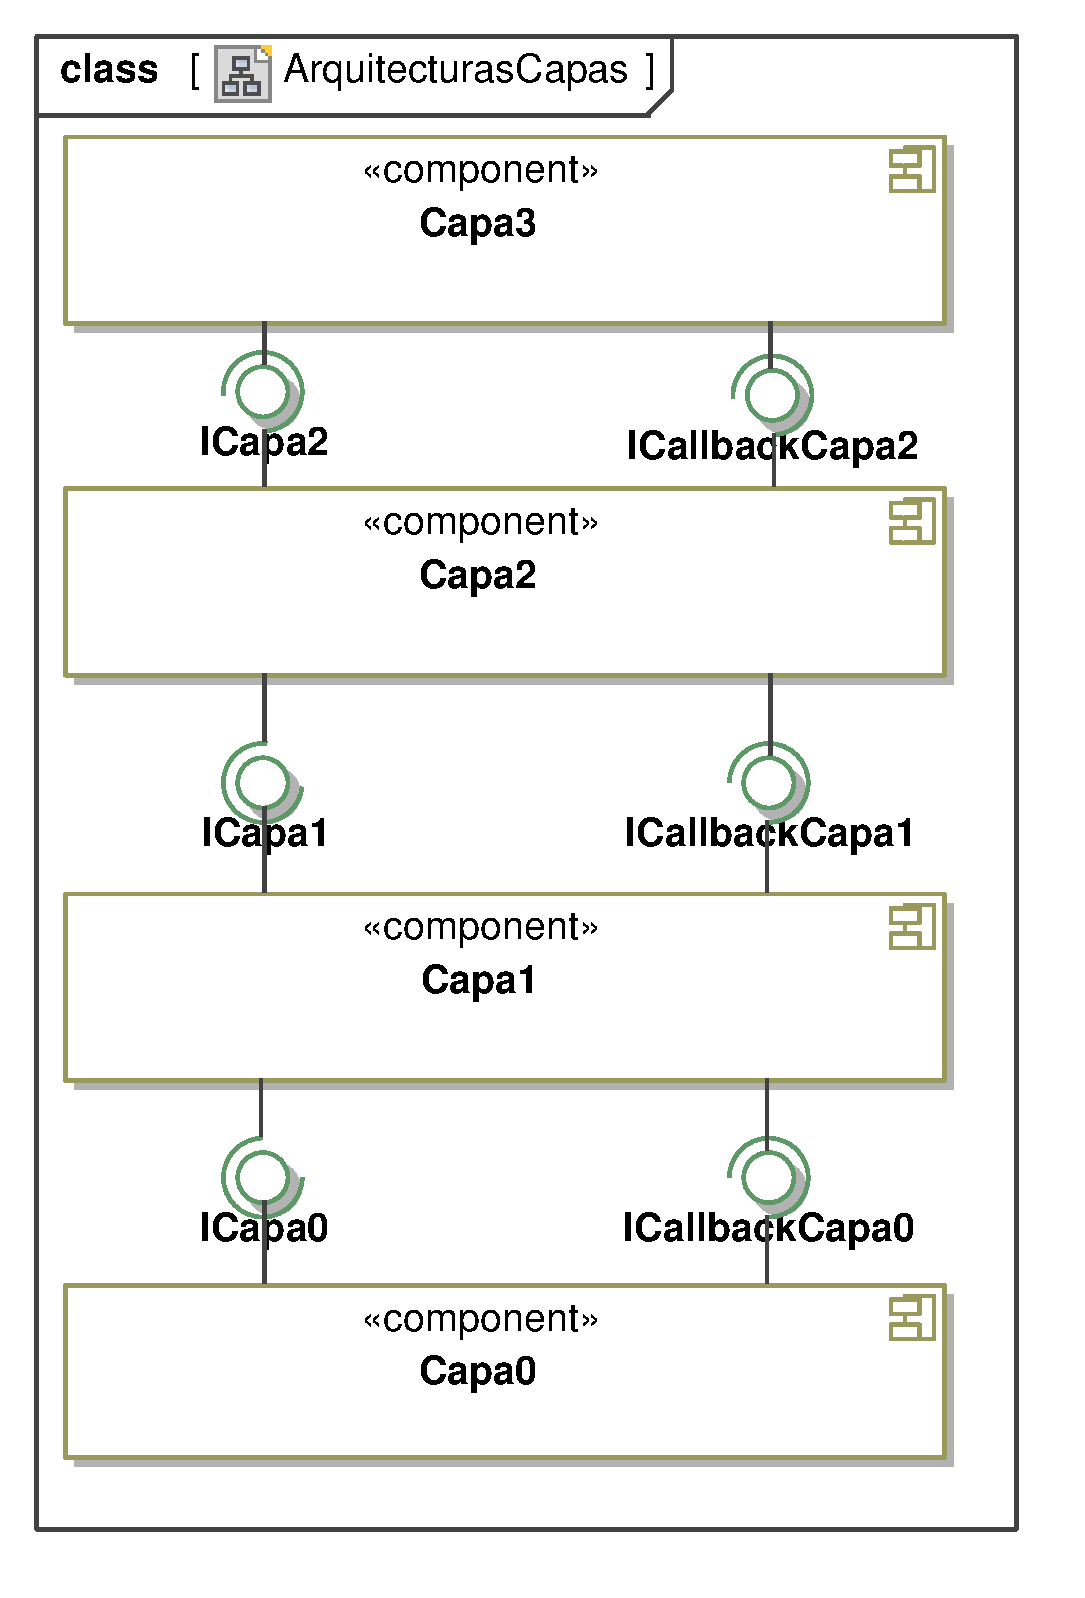
\includegraphics[width=.40\linewidth,keepaspectratio=true]{images/patterns/layered00.eps}
	\end{center}
\end{frame}

\subsection{Sistemas Web}

\begin{frame}[c]
    \frametitle{Sistema Informático Web}
    %% TODO: Buscar una definición mejor o más estandarizada.
    \begin{block}{Sistema Informático Web}
        Un \emph{Sistema Informático Web} es un sistema cliente servidor donde el cliente está codificado utilizando tecnologías web, como HTML, CSS y Javascript, siendo por tanto accesible desde un navegador web; y/o donde el cliente se comunica con el servidor por medio del protocolo HTTP.
    \end{block}
\end{frame}

\begin{frame}[c]
	\frametitle{¿Por qué se utilizan tecnologías Web?}
    \centering \textbf{Ventajas} \\
    \begin{enumerate}
        \item<2-> Multiplataforma.
        \item<3-> Onmipresencia de la web.
        \item<4-> No suelen precisar permisos especiales a nivel de red.
        \item<5-> Facilidad de mantenimiento (código móvil).
        \item<6-> Fuerte estandarización.
        %% Balanceadores de carga
        \item<7-> Favorecen la \emph{recognizability}, reduciendo su curva de aprendizaje.
        \item<8-> Madurez de las herramientas.
    \end{enumerate}
    \uncover<9->{
        \centering \textbf{Inconvenientes} \\
        \begin{enumerate}
            \item<10-> Seguridad.
            %% https://goo.gl/ypz4VD
            \item<11-> Tecnologías originalmente desarrolladas para \emph{hipertexto}.
            \item<12-> Tecnologías lentas.
            \item<13-> Tecnologías dependientes de terceros.
        \end{enumerate}
    }
\end{frame}

\subsection{Arquitecturas Empresariales en Capas}

\subsubsection{Problema a Resolver}

\begin{frame}[c,fragile]
	\frametitle{Sistema Monocapa}
    \begin{lstlisting}[basicstyle=\small]
<% SQLtxt = "SELECT Producto, Cantidad, Precio
               FROM articulos"
   set rs = CreateObject("ADODB.Recordset")
   rs.Open SQLtxt,"DSN=Mibase" %>
<table>
   <% Do While NOT rs.EOF%>
      <tr>
        <td><%= rs("Producto")%></td>
        <td><%= rs("Cantidad")%></td>
        <td align="right">
          <%= FormatCurrency(rs("Precio"))%>
        </td>
      </tr>
   <% rs.MoveNext
      Loop
      rs.Close %>
</table>
    \end{lstlisting}
\end{frame}

\subsubsection{Capas de un SIE}

\begin{frame}[c]
	\frametitle{Arquitectura en Capas de un SIE}
	\begin{center}
        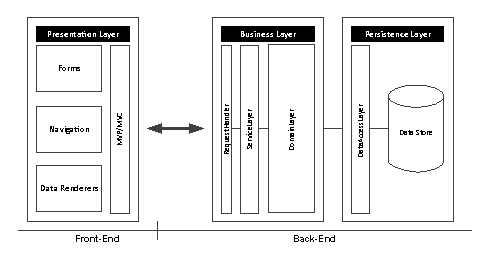
\includegraphics[width=\linewidth,keepaspectratio=true]{images/enterpriseLayers/enterpriseLayers.eps}
	\end{center}
\end{frame}

\begin{frame}[c]
	\frametitle{Responsabilidades de la Capa de Presentación}
	\begin{enumerate}[<+->]
        \item Permitir a los usuarios interactuar con el sistema.
        \item Introducir datos en el sistema (validándolos previamente).
        \item Visualizar los datos de salida de manera amigable al usuario.
        \item Facilitar operaciones simples (filtros, ordenaciones y cambios de formato) sobre los datos.
        \item Facilitar la navegación por el sistema.
        \item Mejorar la experiencia de usuario (UX). %% Hellmans
        \item Gestionar la comunicación con el servidor.
        \item Gestionar situaciones excepcionales.
	\end{enumerate}
\end{frame}

\begin{frame}[c]
	\frametitle{Responsabilidades de la Capa de Negocio}
	\begin{enumerate}[<+->]
        \item Atender las peticiones de los clientes.
        \item Validar las peticiones de los clientes.
        \item Controlar el acceso a los datos.
        \item Asegurar el cumplimiento de \alert{reglas de negocio} existentes.
        \item Asegurar la \alert{transaccionalidad} de las operaciones de negocio.
        \item Recuperar y almacenar datos del almacén o almacenes persistentes.
        \item Facilitar la eficiencia del sistema.
        \item Gestionar la comunicación con los servicios externos.
        \item Ejecutar operaciones (periódicas) del sistema.
        \item Gestionar de manera adecuada casos excepcionales.
        \item Ayudar a mejorar la experiencia de usuario.        
        \item Ayudar a satisfacer requisitos no funcionales.        
	\end{enumerate}
\end{frame}

\begin{frame}[c]
	\frametitle{Responsabilidades de la Capa de Persistencia}
	\begin{enumerate}[<+->]
        \item Almacenar los datos de manera no volátil.
        \item Recuperar datos del almacén persistente,
        \item Asegurar la disponibilidad de los datos.
        \item Controlar la integridad de los datos.
        \item Asegurar un acceso eficiente a los datos.
	\end{enumerate}
\end{frame}

\subsection{Tecnologías de Implementación}

\begin{frame}[c]
	\frametitle{Tecnologías de Implementación ES}
    %%  Dividir en tres imágenes
	\begin{center}
        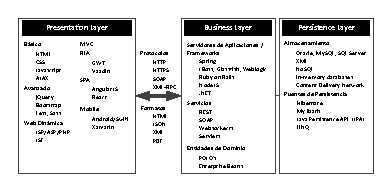
\includegraphics[width=\linewidth,keepaspectratio=true]{images/enterpriseLayers/technologies.eps}
	\end{center}
\end{frame}

\subsection{Distribución de Capas en Arquitecturas Empresariales}

\begin{frame}[c]
	\frametitle{Despliegue de Aplicaciones Empresariales}
	\begin{enumerate}[<+->]
        \item Front-end en el cliente y back-end en uno o más servidores.
        \item Dominio y persistencia pueden ir en el mismo servidor (\emph{two tier}) o en servidores separados (\emph{three tiers}).
        \item Los clientes pueden ser pesados (PCs) o ligeros (Smartphones, tablets).
        \item Trabajo sin conexión puede requerir parte de la capa de dominio (y persistencia) en el cliente.
        \item La capa de presentación puede ser de código fijo (app, desktop) o móvil (HTML + Javascript).
        \item La capa de presentación podría generarse en el servidor y ejecutarse en el cliente (Server Pages).
	\end{enumerate}
\end{frame}

%\section{Capa de Negocio}
%
%\subsection{Problema Común}
%
%\begin{frame}[c]
%    \frametitle{Problema Común a los Patrones de la Capa de Negocio}
%    \begin{block}{Problema Común}
%        El problema común a los patrones de la capa de negocio es donde colocar la
%        lógica de negocio de manera que se satisfagan las responsabilidades de la capa de negocio.
%    \end{block}
%    %% Poner ejemplo común
%\end{frame}
%
%\subsection{Table Module}
%
%\begin{frame}[c]
%    \frametitle{Table Module (obsoleto)}
%    \begin{block}{Solución Table Module}
%        Crear una clase que gestione la lógica de negocio de una tabla (o vista) completa.
%    \end{block}
%    %% Poner ejemplo
%    %% Crear ejemplo en GWT y subirlo a Git.
%\end{frame}
%
%\begin{frame}[c]
%    \frametitle{Table Module (obsoleto)}
%    \centering{\textbf{Ventajas}}
%    \begin{enumerate}
%        \item<2-> Facilidad de uso en lenguajes 4GL.
%    \end{enumerate}
%    \ \\ \ \\
%    \uncover<3->{
%        \centering{\textbf{Desventajas}}
%        \begin{enumerate}
%            \item<3-> Manipula mal instancias en solitario.
%            \item<4-> Dificulta la gestión de datos residentes en varias tablas.
%            \item<5-> Genera problemas de integración con otras aplicaciones.
%            \item<6-> No utiliza orientación a objetos.
%            \item<7-> Crea rápidamente problemas de redundancia en la lógica de negocio.
%            \item<8-> Genera problemas con reglas de negocio complejas.
%        \end{enumerate}
%    }
%\end{frame}

%\begin{frame}
%    \framtitle{\emph{Smart UI Antipattern} }
%
%    %% Put all the business logic into the user interface. Chop the application into
%    %% small functions and implement them as separate user interfaces, embedding
%    %% the business rules into them. Use a relational database as a shared repository of
%    %% the data. Use the most automated UI building and visual programming tools available.
%
%Advantages
%Productivity is high and immediate for simple applications.
%Less capable developers can work this way with little training.
%Even deficiencies in requirements analysis can be overcome by releasing a prototype to users
%and then quickly changing the product to fit their requests.
%Applications are decoupled from each other, so that delivery schedules of small modules can
%be planned relatively accurately. Expanding the system with additional, simple behavior can
%be easy.
%Relational databases work well and provide integration at the data level.
%4GL tools work well.
%When applications are handed off, maintenance programmers will be able to quickly redo
%portions they can't figure out, because the effects of the changes should be localized to each
%particular UI.
%Disadvantages
%Integration of applications is difficult except through the database.
%There is no reuse of behavior and no abstraction of the business problem. Business rules
%have to be duplicated in each operation to which they apply.
%Rapid prototyping and iteration reach a natural limit because the lack of abstraction limits
%refactoring options.
%Complexity buries you quickly, so the growth path is strictly toward additional simple
%applications. There is no graceful path to richer behavior.
%\end{frame}

%\subsection{Transaction Script}
%
%\begin{frame}[c]
%    \frametitle{Transaction Script (obsoleto)}
%    \begin{block}{Solución Transaction Script}
%        Crear un conjunto de funciones que respondan a los eventos que se puedan generar
%        desde la interfaz de usuario, ejecutando para ello la lógica de negocio que sea necesaria.
%    \end{block}
%    %% Poner ejemplo
%    %% Crear ejemplo y subirlo a Git.
%\end{frame}
%
%\begin{frame}[c]
%    \frametitle{Transaction Script (obsoleto)}
%    \centering{\textbf{Ventajas}}
%    \begin{enumerate}
%        \item<2-> Facilidad de implementación en aplicaciones sencillas.
%    \end{enumerate}
%    \ \\ \ \\
%    \uncover<3->{
%        \centering{\textbf{Desventajas}}
%        \begin{enumerate}
%            \item<4-> No utiliza orientación a objetos.
%            \item<5-> Crea rápidamente problemas de redundancia en la lógica de negocio.
%            \item<6-> Genera problemas con reglas de negocio complejas.
%            \item<7-> Genera problemas de evolución.
%        \end{enumerate}
%    }
%\end{frame}
%
%\subsection{Domain Model + Service Layer}
%
%\begin{frame}[c]
%    \frametitle{Domain Model}
%    \begin{block}{Solución Domain Model}
%        Modela el dominio del problema utilizando orientación a objetos y distribuye las reglas de negocio de manera adecuada entre las clases de dominio que corresponda.
%    \end{block}
%    %% Poner ejemplo
%    %% Crear ejemplo y subirlo a Git.
%\end{frame}
%
%\begin{frame}[c]
%    \frametitle{Domain Model}
%    \centering{\textbf{Ventajas}}
%    \begin{enumerate}
%        \item<2-> Orientado a objetos.
%        \item<3-> Permite la utilización de patrones de diseño.
%        \item<4-> Reduce la redundancia de código.
%        \item<5-> Soporta mejor las reglas de negocio complejas.
%        \item<6-> Ofrece una mayor facilidad de evolución.
%    \end{enumerate}
%    \ \\ \ \\
%    \uncover<7->{
%        \centering{\textbf{Desventajas}}
%        \begin{enumerate}
%            \item<8-> Impedancia objeto-relacional u objeto-xxx.
%            \item<9-> Mayor complejidad de diseño e implementación.
%        \end{enumerate}
%    }
%\end{frame}
%
%\begin{frame}[c]
%    \frametitle{Service Layer}
%    \begin{block}{Solución Domain Model}
%        Aislar al modelo de dominio de otras capas y aplicaciones mediante la creación de una capa de servicio que:
%        \begin{enumerate}
%            \item Especifique las operaciones a las cuales el modelo de dominio es capaz de responder.
%            \item Permita redirigir peticiones a las operaciones del modelo de dominio que corresponda, devolviendo la respuesta que corresponda.
%            \item Permite encapsular la \emph{lógica de la aplicación} o \emph{workflow}.
%        \end{enumerate}
%    \end{block}
%\end{frame}
%
%\begin{frame}[c]
%    \frametitle{Service Layer}
%    \begin{block}{Lógica de la Dominio}
%        La \emph{lógica de dominio} es el conjunto de procedimientos, restricciones y normas que rigen el funcionamiento de una determinada organización o dominio, y que son independientes de la existencia o no de una aplicación software.
%    \end{block}
%    \uncover<2->{
%        \begin{block}{Lógica de la Aplicación}
%            La \emph{lógica de la aplicación} es el conjunto de procedimientos, restricciones y normas que rigen el funcionamiento de una determinada aplicación. Es la encargada de gestionar elementos como transacciones, accesos a almacenes persistentes o seguridad.
%        \end{block}
%    }
%\end{frame}
%
%\begin{frame}[c]
%    \frametitle{Service Layer}
%    \begin{enumerate}
%        \item<1-> Aisla al modelo de dominio de servicios concretos.
%        \item<2-> Favorece la gestión de la lógica de la aplicación.
%        \item<3-> Favorece la gestión de la concurrencia.
%    \end{enumerate}
%\end{frame}
%
%\section{Domain-Driven Design}
%
%\subsection{Introducción}
%
%\begin{frame}[c]
%    \frametitle{Domain-Driven Design}
%     \begin{block}{Domain-Driven Design}
%        \alert{\emph{Domain-Driven Design}} es una técnica de desarrollo sw donde todo el diseño de un producto sw gira en torno a un elemento central y fundamental que es el \emph{modelo de dominio}, el cual captura el dominio y la lógica de negocio de dicho producto sw.
%     \end{block}
%      %% Contar la historia de Monty Python
%      %% Contar la historia del PCB
%      %% Ventajas e Incovenientes: https://goo.gl/gPx5DE
%
%      %% Add Page 8 documento de Evans.
%\end{frame}
%
%%%\begin{frame}[c]
%%%    \frametitle{Domain-Driven Design}
%%%     \begin{block}{Ubiquitous Language}
%%%
%%%     \end{block}
%%%     %% Leer Capítulo 3 de Evans
%%%\end{frame}
%%
%\subsection{Entities}
%
%\begin{frame}[c]
%    \frametitle{Entities}
%     \begin{block}{Entity}
%        Una \emph{entity} es un objeto del dominio con una identidad y un ciclo de vida que debe ser reconocido y monitorizados.
%     \end{block}
%     \uncover<2->{
%         \begin{block}{Características de un Identificador}
%            %% Olvidarse del problema de las claves surrogadas de las bases de datos relacionales.
%            \begin{enumerate}
%                \item<3-> Únicos para cada objeto e inmutables.
%                \item<4-> Pueden ser un único atributo o combinación de atributos.
%                \item<5-> Si no se encuentra un identificador natural, puede ser generado por la aplicación.
%                \item<6-> Si son generados, se esconden (normalmente) al usuario.
%            \end{enumerate}
%         \end{block}
%     }
%     %% Ejemplo de asiento en función numerada y no numerada.
%     %% "Beyond identity issues, entities tend to fulfill their responsabilities
%     %% by coordinating the operations of the objects they own"
%\end{frame}
%
%\subsection{Value Objects}
%
%\begin{frame}[c]
%    \frametitle{Value Objects}
%    \begin{block}{Value Object}
%        Elementos del dominio sin identidad definida, cuya existencia no es necesario monitorizar, y que simplemente representan valores de alguna propiedad de una entidad.
%        %% Si me dan otro objeto, no tiene porque ser exactamente el mismo, me vale con que tenga
%        %% sus mismas propiedades.
%    \end{block}
%    \uncover<2->{
%         \begin{block}{Características de un \emph{Value Object}}
%            %% Olvidarse del problema de las claves surrogadas de las bases de datos relacionales.
%            \begin{enumerate}
%                \item<3-> Dos instancias con los mismos valores se consideran idénticas, aunque tengan identidades distintas.
%                \item<4-> Se recomienda hacer los \emph{value objects} inmutables.
%            \end{enumerate}
%        \end{block}
%     }
%\end{frame}
%
%\subsection{Services}
%
%\begin{frame}[c]
%    \frametitle{Services}
%    \begin{block}{Service}
%        Un \emph{service} encapsula operaciones de dominio que no son responsabilidad natural de ninguna \emph{entity} o \emph{value object}.
%    \end{block}
%    \uncover<2->{
%         \begin{block}{Características de un \emph{Service}}
%            %% Declaración trimestal del IVA.
%            \begin{enumerate}
%                \item<3-> Forma parte del \emph{lenguaje universal} del dominio.
%                \item<4-> Su interfaz está definida en base a otros elementos del modelo de dominio.
%                \item<5-> Su operación u operaciones no tienen estado (\emph{stateless}).
%            \end{enumerate}
%        \end{block}
%     }
%\end{frame}
%
%\subsection{Aggregates}
%
%\begin{frame}[c]
%    \frametitle{Aggregates}
%    \begin{block}{Aggregate}
%        Un \emph{aggregate} es un conjunto cohesionado de \emph{entities} y \emph{value objects} con una frontera clara con el resto del modelo de dominio y un conjunto de invariantes bien definidos que deben preservarse dentro de dicho conjunto.
%    \end{block}
%    \uncover<2->{
%        \begin{block}{Aggregate Root}
%            Dentro de un \emph{aggregate}, el \emph{aggregate root} es una \emph{entity} que controla el ciclo de vida del resto de los elementos del \emph{aggregate} y que contiene la información necesaria para encargarse de la preservación de los invariantes.
%        \end{block}
%    }
%\end{frame}
%
%\begin{frame}[c]
%    \frametitle{Características de los \emph{Aggregates}}
%    \begin{enumerate}[<+->]
%        %% Alumno y expediente
%        \item El \emph{aggregate root} debe tener identidad global.
%        \item El resto de elementos del \emph{aggregate} sólo necesita tener identidad local.
%        \item El \emph{aggregate root} es el encargado de preservar los invariantes.
%        \item El tiempo de vida de un \emph{aggregate} debe ser uniforme a sus miembros.
%        \item Los elementos externos al \emph{aggregate} sólo deben referenciar al \emph{aggregate root}.
%        \item Los elementos internos de un \emph{aggregate} sólo pueden referenciar como elementos externos \emph{aggregate roots}.
%        \item Los elementos internos de un \emph{aggregate} sólo deben utilizarse de manera transitoria fuera del \emph{aggregate}.
%        \item Sólo los \emph{aggregate roots} pueden ser recuperados de persistencia.
%        \item Si se elimina un \emph{aggregate root}, se debe eliminar todo el \emph{aggregate}.
%    \end{enumerate}
%\end{frame}
%
%\subsection{Repositories}
%
%\begin{frame}{c}
%    \frametitle{Repositories}
%    \begin{block}{Repository}
%        Un \emph{repository} representa una clase que, a nivel conceptual, representa una colección con todas las instancias de una determinado elemento del dominio. El repositorio debe además proporcionar métodos para recuperar conjuntos de instancias concretos dentro de dicha colección, añadir nuevas instancias o eliminarlas.
%    \end{block}
%\end{frame}
%
%\begin{frame}[c]
%    \frametitle{Características de los \emph{Repositories}}
%    \begin{enumerate}[<+->]
%        %% Alumno y expediente
%        \item Sólo existirán \emph{repositories} para los \emph{aggregates root}.
%        \item Normalmente, existirá un \emph{repository} por cada \emph{aggregate root}.
%        \item Cada \emph{repository} contendrá las operaciones CRUD básicas, más un método para recuperar todas las instancias de un elemento del dominio.
%        \item Además, cada \emph{repository} contendrá otros métodos de búsqueda o cálculo siempre y cuando sean necesarios.
%        %% Ojo con los repositorios, no son mágicos.
%    \end{enumerate}
%\end{frame}
%
%\subsection{Otros elementos DDD}
%
%\begin{frame}[c]
%    \frametitle{Otros elementos DDD}
%    \begin{enumerate}[<+->]
%        \item Domain Events.
%        \item Modules.
%        \item Factories.
%    \end{enumerate}
%\end{frame}

% \subsection{Identificación de Entidades}

%%\begin{frame}[c]
%%    \frametitle{Características de los Identificadores}
%%    \begin{itemize}
%%        \item Inmutables.
%%        \item Significativos.
%%    \end{itemize}
%%    %% Copiar de Fowler.
%%
%%    Ids.
%%
%%    - Únicos para cada objeto.
%%    - Un único atributo o combinación de atributos.
%%    - Artificial, generado por la aplicación (ojo con los sistemas distribuidos o interconectados)
%%    - Inmutables
%%    - IDs artificiales pueden esconderse al usuario.
%%    -
%%\end{frame}
%
%%\begin{frame}[c]
%%    \frametitle{Claves Naturales vs Claves Surogadas}
%%    %% Copiar de Fowler.
%%\end{frame}
%


%\section{Sumario y Referencias}
%
%\begin{frame}[c]
%    \frametitle{¿Qué Tengo que Saber de Todo Esto?}
%    \begin{enumerate}[<+->]
%        \item TODO
%    \end{enumerate}
%\end{frame}

%\subsection{Referencias}
%
%\begin{frame}
%	\frametitle{Referencias}
%    \nocite{}
%	\bibliographystyle{apalike}
%    \bibliography{arqEmp}
%\end{frame}

\end{document}
